\documentclass{article}

\usepackage[portuguese]{babel}

\usepackage{amsmath, amssymb}
\usepackage{graphicx}
\usepackage[colorlinks=true, allcolors=blue]{hyperref}

\usepackage[section]{placeins}

\title{Lista 03}
\author{Vinícius de Oliveira Peixoto Rodrigues (245294)}
\date{Setembro de 2022}

\begin{document}
\maketitle

\section*{Questão 1}

O problema principal é que o modo ECB deixa a desejar em difusão. Se um plaintext contém muitas regiões com valores iguais, todas elas terão o mesmo output em ciphertext, de modo que o ECB falha em difundir as propriedades estatísticas do plaintext.

Um exemplo visual e particularmente grave é a encriptação de imagens (onde é comum ter regiões relativamente grandes e com a mesma cor) no modo ECB:

\FloatBarrier
\begin{figure}[!ht]
    \begin{center}
        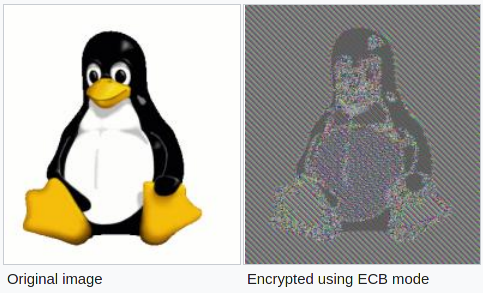
\includegraphics[width=\textwidth]{images/ecb_image.png}
    \end{center}
\end{figure} 

Percebe-se que as regiões (suficientemente grandes) de mesma cor na imagem original continuam com a mesma cor na imagem encriptada.

\newpage
\section*{Questão 2}

\FloatBarrier
\begin{figure}[!ht]
    \begin{center}
        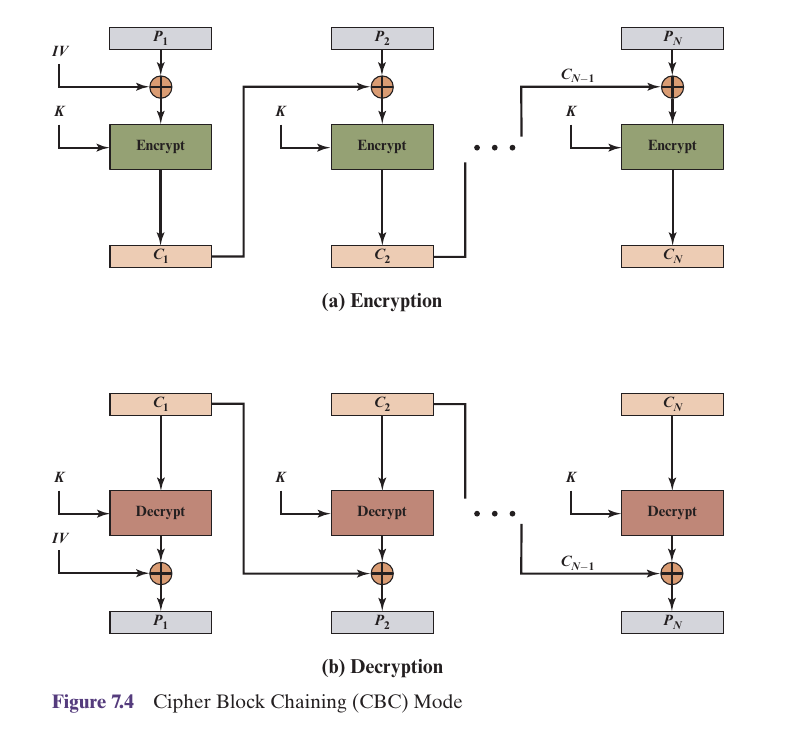
\includegraphics[width=\textwidth]{images/cbc_mode.png}
    \end{center}
\end{figure} 

A figura acima mostra um diagrama do modo CBC. Em termos de paralelização, percebe-se imediatamente que:

\begin{itemize}
    \item O modo de encriptação \textbf{não é paralelizável}, visto que a cifra $C_i$ necessariamente depende do resultado da cifra $C_{i-1}$ (elas estão relacionadas por $C_i = E(K, C_{i-1} \oplus P_i)$)
    \item O modo de decriptação \textbf{é paralelizável}, visto que cada $P_i$ só depende de $C_{i-1}$ e a stream $C_1, C_2, ...$ é conhecida por inteiro ($P_i = D(K, C_i) \oplus C_{i-1}$), de modo que as decriptações podem ser feitas independentemente
\end{itemize}

\newpage
\FloatBarrier
\begin{figure}[!ht]
    \begin{center}
        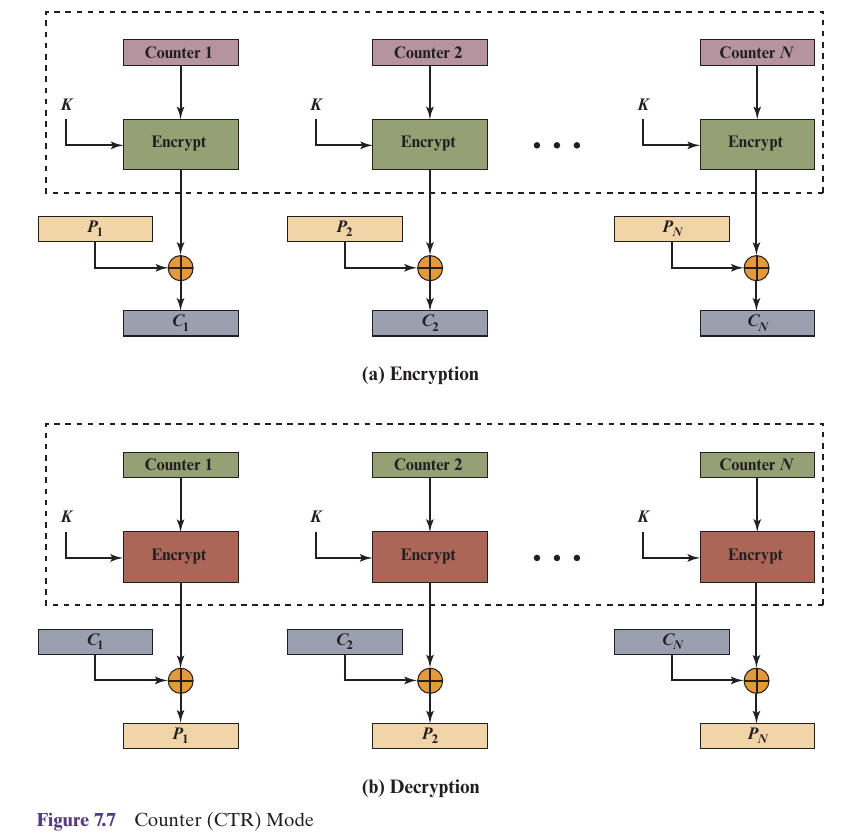
\includegraphics[width=\textwidth]{images/ctr_mode.png}
    \end{center}
\end{figure} 

A figura acima mostar um diagrama do modo CTR. Nesse caso, em termos de paralelização tem-se que:

\begin{itemize}
    \item O modo de encriptação \textbf{é paralelizável}, visto que os valores de $C_i$ dependem só de $T_i$ (\texttt{Counter i}), que são conhecidos e normalmente são $T_i = \texttt{nonce + i}$ ($C_i = P_i \oplus E(K, T_i)$)
    \item O modo de decriptação \textbf{também é paralelizável}, visto que, novamente, os valores $P_i$ dependem só de $T_i$ ($P_i = C_i \oplus E(K, T_i)$)
\end{itemize}

Vale notar também que no modo CTR só é necessário usar o modo de encriptação do algoritmo de block cipher.

Desse modo, o CTR, que permite paralelização tanto da encriptação quanto da decriptação, apresenta clara vantagem sobre o CBC, que só permite paralelização na decriptação.

\newpage
\section*{Questão 3}

O esquema CBC-MAC é um algoritmo para gerar um MAC (\textit{Message Authentication Code}) a partir de uma block cipher em modo CBC (o MAC é o último bloco de ciphertext):

\FloatBarrier
\begin{figure}[!ht]
    \begin{center}
        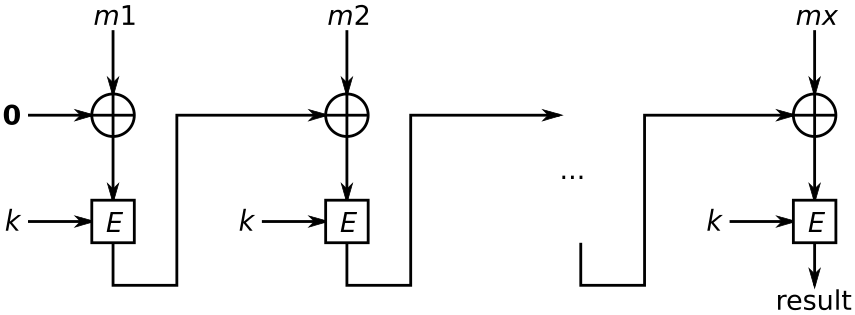
\includegraphics[width=\textwidth]{images/cbc_mac.png}
    \end{center}
\end{figure} 

O modo CCM (\textbf{C}ounter with \textbf{C}BC-\textbf{M}AC) funciona em um esquema de "\textit{authenticate-then-encrypt}", de modo que é inicialmente calculado um MAC para a mensagem, e em seguida a mensagem + MAC são cifradas usando uma block cipher no modo CTR.

Algumas vantagens do modo CCM são:

\begin{itemize}
    \item Garante a integridade da mensagem, além de prover a encriptação
    \item O aumento no tamanho da mensagem devido à funcionalidade de checagem de integridade é muito pequeno
    \item O modo CCM tem segurança confirmada matematicamente (desde que o \texttt{nonce} do CTR não seja reutilizado e que sejam usadas chaves diferentes para encriptação e autenticação)
    \item Toma vantagem do modo CTR, exigindo somente um modo de operação (encriptação ou decriptação)
\end{itemize}

\section*{Questão 4}

A ideia básica do algoritmo é tomar vantagem do teorema de Euler:

\begin{equation*}
    a^{\varphi(n)} \equiv 1 \mod n
\end{equation*}

para encontrar números $(e, d, n)$ que satisfaçam 

\begin{equation*}
    (m^d)^e \equiv m \mod n
\end{equation*}

ou, equivalentemente,

\begin{equation*}
    (m^e)^d \equiv m \mod n
\end{equation*}

O número $n$ é definido como $n = pq$, com $p$, $q$ sendo primos muito grandes. Isso implica que $\varphi(n) = (p-1)(q-1)$.

Note que pelo teorema de Euler,

\begin{equation*}
    m^{\varphi(n)} \equiv 1 \mod n \Rightarrow m^{k\varphi(n)} \equiv 1 \mod n \Rightarrow m^{k\varphi(n) + 1} \equiv m \mod n
\end{equation*}

Portanto, se $m^{ed} \equiv m \mod n$, temos

\begin{equation*}
    ed = k\varphi(n) + 1 \Rightarrow ed \equiv 1 \mod \varphi(n)
\end{equation*}

Daí, é escolhido um valor para $e$ (normalmente se escolhe o primo $e = 2^{16} + 1$) e em seguida é calculado $d$ (i.e. o inverso multiplicativo modular de $e$) usando-se o algoritmo de Euclides estendido. É importante que $gcd(e, \varphi(n)) = 1$ para garantir que $m^e \equiv 1 \mod n$ seja uma bijeção.

Finalmente, tendo em mãos valores $(e, d, n)$ que satisfazem $(m^e)^d \equiv m \mod n$, o processo de cifração/decifração é imediato:

\begin{itemize}
    \item cifração: $C = P^e \mod n$
    \item decifração: $P = C^d \mod n = (P^e)^d \mod n = P \mod n = P$
\end{itemize}

Portanto, o passo-a-passo da geração de chaves é:

\begin{itemize}
    \item Escolha primos $p$ e $q$ grandes
    \item Calcule $n = pq$
    \item Calcule $\varphi(n) = (p-1)(q-1)$
    \item Escolha $e$ tal que $gcd(e, \varphi(n)) = 1$
    \item Calcule $d$ como solução de $d \equiv e^{-1} \mod \varphi(n)$
\end{itemize}

Daí, $K_{pu} = (e, n)$ e $K_{pr} = (d, n)$.

\section*{Questão 5}

\subsection*{Item (a)}

Deve satisfazer a condição $ed \equiv 1 \mod \varphi(n)$.

\subsection*{Item (b)}

O que mitiga o risco (e também é a principal força do RSA) é a seleção de primos aleatórios em $n = pq$; a chance de se encontrar um par fixo $(e,d)$ que satisfaz $ed-1 \equiv 0 \mod (p_1-1)(q_1-1) \equiv 0 \mod (p_2-1)(q_2-1)$ é muito pequena. Na prática, é muito mais comum investigar vulnerabilidades onde são geradas chaves $n$ que compartilham um fator primo.

\section*{Questão 6}


\section*{Questão 7}

Não. Na prática, quebrar o RSA exige fatorar o fator $n$, e os algoritmos mais rápidos de fatoração levam tempo proporcional a $exp(\sqrt{\ln n \cdot \ln(\ln n))} \approx 4 \cdot 10^{29}$ para $n$ de 1024 bits (essa é uma estimativa extremamente otimista). No AES, um ataque por força bruta consiste em testar todas as combinações de chaves; $2^{128} \approx 3 \cdot 10^{38}$. Desse modo, apesar de o RSA usar chaves mais longas, a estimativa de tempo necessário para quebrá-lo não chega a ser maior do que a do AES128.

\section*{Questão 8}

A maneira mais eficaz seria, naturalmente, fatorar o módulo $n$, mas isso é impraticável para valores grandes. Ataques mais comuns envolvem erros no uso do RSA, como por exemplo:

\begin{itemize}
    \item Se é sabido que dois pares de chaves possuem um fator primo em comum, é possível fatorar o módulo $n$ usando o algoritmo de Euclides
    \item Se o módulo $n$ for reutilizado (gerando-se apenas pares distintos $(e_i,d_i)$ para vários usuários), um dos usuários pode usar o seu par $(e,d)$ para fatorar $n$ e então encontrar as chaves privadas de todos os outros usuários a partir de suas chaves públicas.
    \item Se o expoente privado for pequeno (o que é evidenciado por um expoente público grande), é possível quebrar a chave $d$ relativamente rápido (Wiener attack)
\end{itemize}

\section*{Questão 9}

Certificados digitais são documentos eletrônicos que provam a validade de uma chave pública. Esses documentos são criados e utilizados da seguinte forma:

\begin{itemize}
    \item Uma entidade pede a uma autoridade certificadora a emissão de um certificado e fornece seu ID $A$ e chave $K_{pu}^{A}$
    \item A autoridade gera um documento contendo o ID e a chave pública da entidade, assim como a validade do certificado, e o encripta usando a sua chave privada $K_{pr}^{\text{auth}}$; esse é o certificado: $E(K_{pr}^{\text{auth}}, (T, A, K_{pu}^A))$
    \item A entidade fornece o seu certificado criptografado para third-parties, que por sua vez decriptam o documento usando a chave pública da autoridade certificadora e simultaneamente verificam a validade da autenticação do certificado e obtém os dados da entidade A
\end{itemize}

\section*{Questão 10}

\subsection*{Item (a)}

\begin{itemize}
    \item A criptografia assimétrica resolve (parcialmente) o problema da distribuição de chaves, sendo necessárias apenas $N$ (em vez de $N^2$) chaves públicas (e $N$ privadas) para que $N$ entidades possam se comunicar de forma segura entre si
    \item A criptografia assimétrica permite a verificação de autenticidade de dados, e pode ser usada como uma forma de assinatura digital
\end{itemize}

\subsection*{Item (b)}

Há várias razões:

\begin{itemize}
    \item A criptografia simétrica é simples e fácil de implementar, tendo suporte em hardware nas arquiteturas modernas de processadores mais relevantes (x86, ARM)
    \item Ela é também significativamente mais rápida (importante para aplicações de baixa latência) e ocupa menos espaço (tamanho de chaves menor, ciphertext com mesmo tamanho que plaintext)
    \item Em várias aplicações ela faz mais sentido do que a assimétrica (por exemplo, criptografia de unidades de armazenamento)
    \item Ela é (presumidamente) resistente a ataques quânticos (principalmente os baseados na QFT, Quantum Fourier Transform)
\end{itemize}

\end{document}

